\documentclass{article}
\usepackage{parskip}
\usepackage{listings}
\usepackage{pdfpages}
\usepackage{amsmath}
\usepackage[margin=.6in]{geometry}
\begin{document}
\includepdf[pages=10]{Module6}
\includepdf[pages=11]{Module6}
\includepdf[pages=12]{Module6}
Databases record everything in log files. You can log queries, user access, errors/warnings, and performance metrics. 

\includepdf[pages=13]{Module6}
We want to be able to make sure that the full transaction happens or nothing happens. Dying half way through is reeeeaaaalllly bad.

\includepdf[pages=14-19]{Module6}
\includepdf[pages=21-28]{Module6}
\includepdf[pages=29]{Module6}
\includepdf[pages=30]{Module6}
For all databases such that the two databases differ only in one record an algorithm that protects info is differentially private if for all possible outputs the quotient probability that each of the databases will return some data point is bounded by some epsilon. 

Usually differential privacy is acheived by adding noise to the results returned. Its actually pretty hard to implement because there are some queries you don't want any noise in.

\includepdf[pages=31]{Module6}

\includepdf[pages=33]{Module6}
An element can basically be anything in the database and we can associate different security levels with them. 

\includepdf[pages=34]{Module6}
Basically this is all the stuff you learned about when you were doing all that stuff with latices and such. Weeee review.

\includepdf[pages=35]{Module6}
\includepdf[pages=36]{Module6}
Very few people implement multilevel security, so it really only works in theory. The best that people do is to just have separate databases that we encrypt. 

\includepdf[pages=37]{Module6}
We want our encryption to still allow very fast access to the database so we can search and return things with little delay.

\includepdf[pages=38]{Module6}
\includepdf[pages=39]{Module6}


\includepdf[pages=41]{Module6}
\includepdf[pages=42]{Module6}
\includepdf[pages=43]{Module6}
\includepdf[pages=44]{Module6}
\includepdf[pages=45-66]{Module6}












\end{document}